\begin{center}
\textbf{
\MakeUppercase{Приложение А}\\
(обязательное)\\
Исходный код}
\end{center}
\addcontentsline{toc}{section}{Приложение А~(обязательное) Исходный код}

\lstinputlisting{inc/src/result_listing.swift}

\newpage

\begin{center}
\textbf{
\MakeUppercase{Приложение Б}\\
(информационное)\\
Проверка в~системе <<Антиплагиат>>}
\end{center}
\addcontentsline{toc}{section}{Приложение Б (информацинное) Проверка в~системе <<Антиплагиат>>}

\newpage
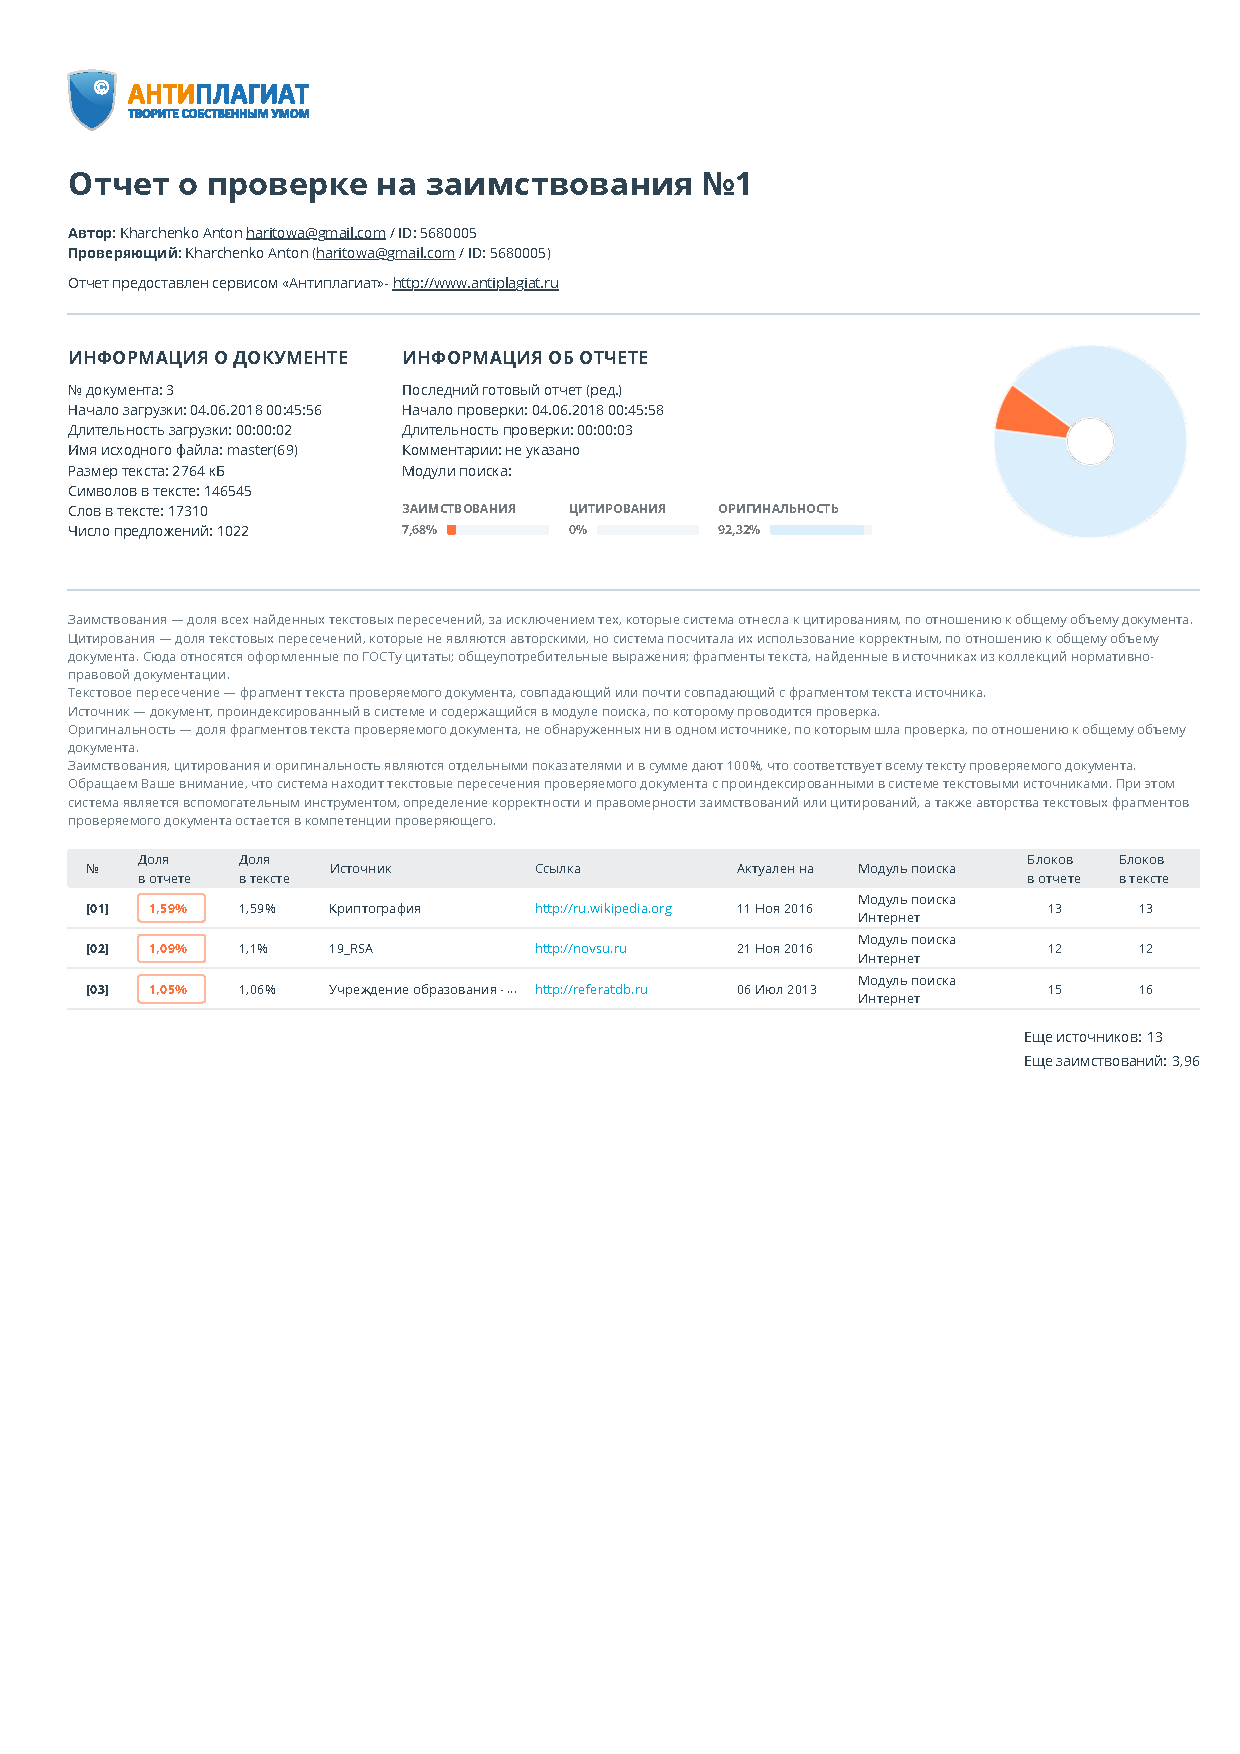
\includepdf[scale=0.9, pages=-,pagecommand={},angle=90]{inc/pdf/antiplagiat.pdf}

\newpage


\begin{center}
\textbf{
\MakeUppercase{Приложение В}\\
(обязательное)\\
Ведомость дипломного проекта}
\end{center}
\addcontentsline{toc}{section}{Приложение В~(обязательное) Ведомость дипломного проекта}

\newpage
\pagestyle{empty}
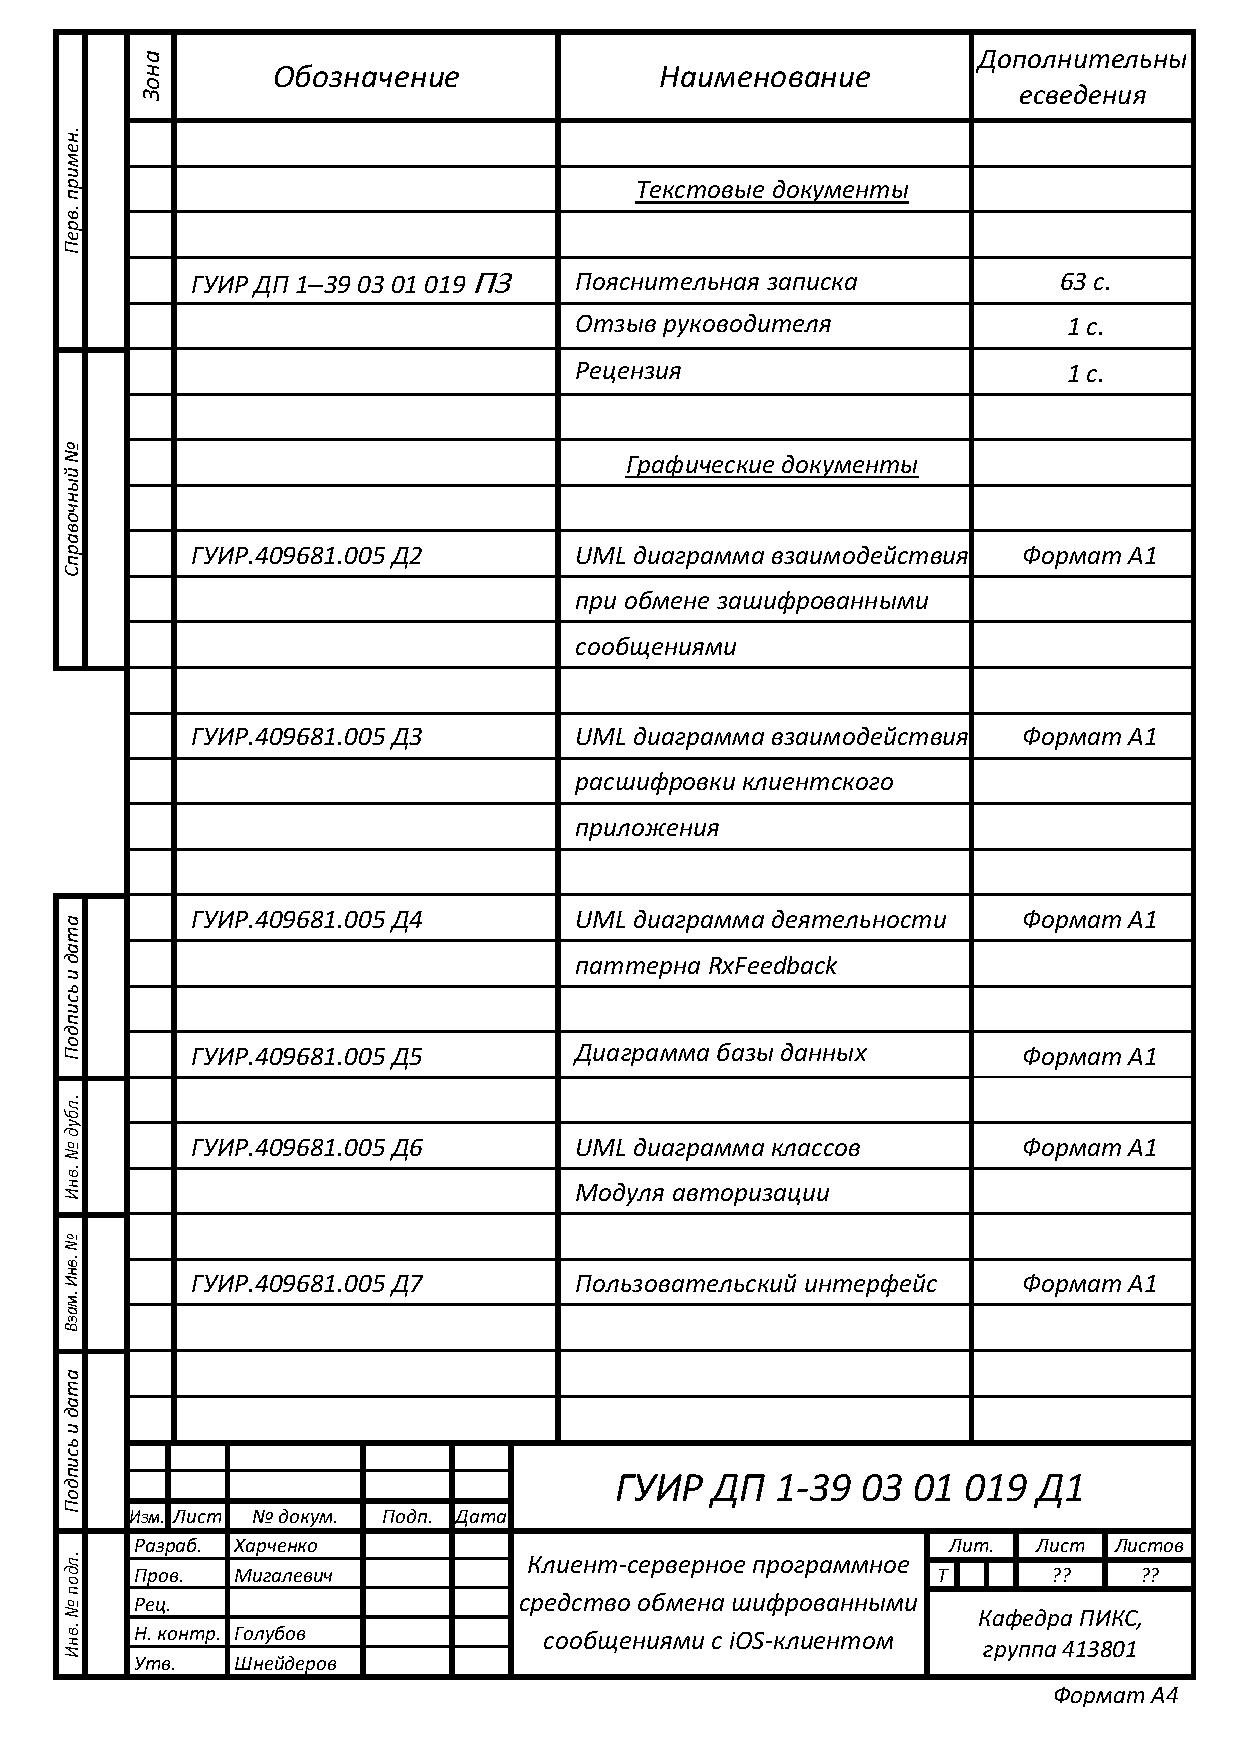
\includepdf[pages=-,pagecommand={}]{inc/pdf/vedomost.pdf}
\pagestyle{fancy}